\documentclass[12pt]{article}

\usepackage[english]{babel}
\usepackage[a4paper,top=2cm,bottom=2cm,left=3cm,right=3cm,marginparwidth=1.75cm]{geometry}
\usepackage{listings}
\usepackage{graphicx}
\usepackage{float}
\usepackage{xcolor}
\usepackage{amsmath}
\usepackage[parfill]{parskip}
\usepackage[colorlinks=true, allcolors=blue]{hyperref}

\definecolor{blue-ncs}{rgb}{0.0, 0.53, 0.74}
\definecolor{alizarin}{rgb}{0.82, 0.1, 0.26}
\definecolor{dkgreen}{rgb}{0,0.6,0}

\lstset{
    basicstyle=\ttfamily\footnotesize,
    keywordstyle=\color{blue-ncs},
    stringstyle=\color{alizarin},
    commentstyle=\color{dkgreen},
    showstringspaces=false,
    frame=single,
    breaklines=true,
}

\begin{document}

\begin{titlepage}
   \begin{center}

       \textbf{UNIVERSITY OF SCIENCE AND TECHNOLOGY OF HANOI}

       \footnotesize{\textbf{DEPARTMENT OF INFORMATION AND COMMUNICATIONS TECHNOLOGY}}
       
       \includegraphics[width=0.4\textwidth]{logo USTH.png}
            
       \vspace{6cm}
       
       \centerline{\hbox to 13cm{\hrulefill}}
       \vspace{-0.1cm}
       {\sc 
       \uppercase{{Distributed Sytem - Practical 2}}

       \vspace{0.1cm}

       \LARGE
       \uppercase{{\textbf{RPC File Transfer}}}}
       \centerline{\hbox to 13cm{\hrulefill}}

       \vspace{9cm}

       By

       Truong Hoang Khanh Linh - 22BI13254
            
   \end{center}
\end{titlepage}

\section{Design}

The RPC service is built using Python’s xmlrpc module, XML-RPC. The service enable remote communication between a client and a server over HTTP. It provides service for file transfer operations.
\begin{itemize}
    \item The client can send or download a file to the server.
    \item The sesrver listens for incoming client requests from the client and processes them.
\end{itemize}

Below is a architecture diagram for XML-RPC:
\begin{figure}[!ht]
\centering
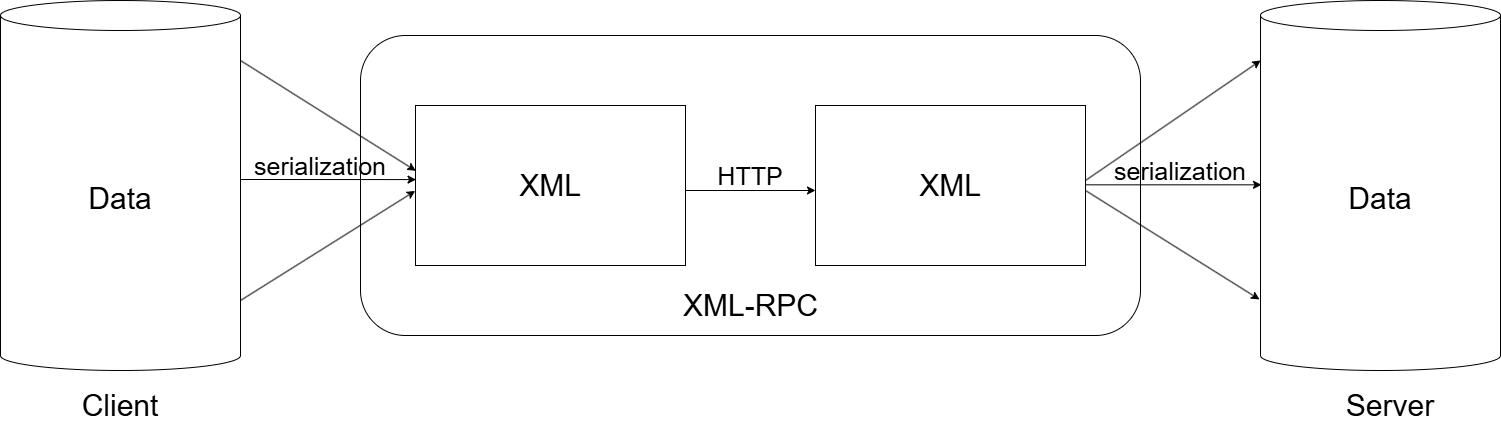
\includegraphics[scale=0.3]{xml-rpc-architecture.png}
\caption{XML-RPC Architecture}
\end{figure}


\section{System organization}
The system follows a client-server architecture, with them communicating over XML-RPC.

\begin{itemize}
    \item The server
\end{itemize}
The server hosts the file transfer service and listens on port 888. Its provides RPC functions to receive the file and return the requested file from the client. Received files are managed locally.

\begin{itemize}
    \item The client
\end{itemize}
The client connects to the server through the server URL link. It offers two functions for file transfer service: to read a local file and send it to the server, to request a file from the server and save it locally.

\newpage

\begin{figure}[!ht]
\centering
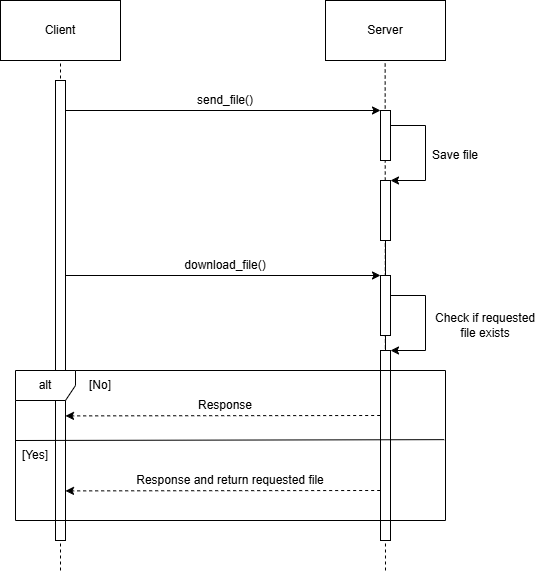
\includegraphics[scale=0.5]{work-flow.png}
\caption{Work Flow of the system}
\end{figure}


\section{Implementation}
The system is implemented in Python using RPC. The client and the server transfer files over XML-RPC.

\subsection{The client}

To send a file to the server, the client runs the \verb|download_file()| function, passing the filename and the file content in binary mode. It wraps the content using \textbf{xmlrpc.client.Binary()} to ensure the transmission of binary data over the XML-RPC protocol.

To download a file from the server, the client requests a file by calling \verb|download_file()| with the desired filename. If the download is successful, the downloaded file is saved locally with a specified name.
\newpage

\begin{lstlisting}[language=Python]
import xmlrpc.client

def send_file(server_url, filename):
    with open(filename, 'rb') as file:
        file_content = file.read()

    proxy = xmlrpc.client.ServerProxy(server_url)   # Create an XML-RPC server proxy

    # Send the file to the server
    response = proxy.send_file(filename, xmlrpc.client.Binary(file_content))
    print(response)


def download_file(server_url, request_filename, save_as):
    proxy = xmlrpc.client.ServerProxy(server_url)

    # Request the file to download from the server
    file_content, message = proxy.download_file(request_filename)
    
    # Save the downloaded file
    if file_content.data:
        with open(save_as, 'wb') as file:
            file.write(file_content.data)
    print(message)


if __name__ == "__main__":
    server_url = "http://192.168.86.128:888"

    download_file(server_url, "file_to_download.txt", "downloaded_file")
    send_file(server_url, "file_to_send.txt")

\end{lstlisting}


\subsection{The server}
The server receives the file transferred from the client with \verb|send_file()|, saves it locally as \verb|\received_file|, and returns a success message to the client.

After receiving the request to download file from the client, the server first checks for the file's existence. If the file exists, it reads the requested file content in binary mode, wraps the content using \textbf{xmlrpc.client.Binary()} and then sends it back to the client along with a success message. If the file does not exist, it will return an message indicating the error.

Below is the code for the server:
\newpage
\begin{lstlisting}[language=Python]
import xmlrpc.server
import os

def send_file(filename, file_content):
    # Save the received file
    with open('received_file', 'wb') as file:
        file.write(file_content.data)
    print(f"File received and saved as 'received_file'.")
    return "File sent successfully."


def download_file(filename):
    # Check if the requested file exists
    if not os.path.exists(filename):
        return "File does not exist."

    with open(filename, 'rb') as file:
        file_content = file.read()
    print(f"Requested file sent successfully.")
    return xmlrpc.client.Binary(file_content), "File downloaded successfully."


if __name__ == "__main__":
    server = xmlrpc.server.SimpleXMLRPCServer(("192.168.86.128", 888))

    # Register the functions with the XML-RPC server
    server.register_function(send_file, "send_file")
    server.register_function(download_file, "download_file")

    print("Server listening on port 888...")

    # Start the server
    server.serve_forever()
\end{lstlisting}


\section{Testing}
First, run \textbf{server.py} to set up the server, let it listen to connections on port 888.
\begin{figure}[!ht]
\centering
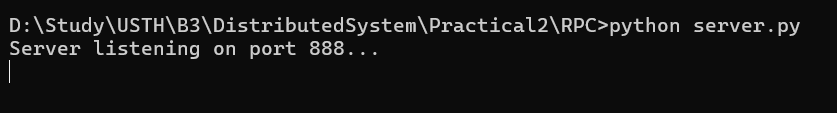
\includegraphics[scale=0.5]{test-server-1.png}
\end{figure}

After that, run \textbf{client.py} to connect the client to the server. Once the connection is established, the client will transfer file to the server and download file from the server at the same time. 

Files are now transfered successfully as shown in the images below.

\begin{figure}[H]
    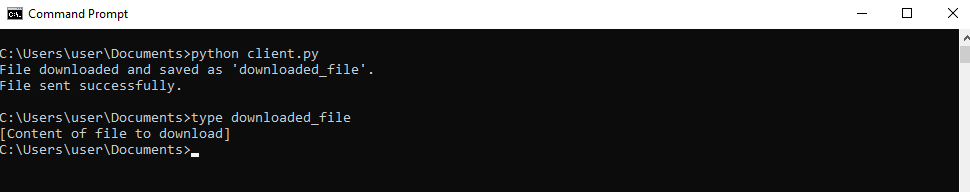
\includegraphics[scale=0.6]{test-client.png}
\end{figure}

\vspace{-0.7cm} % Adjust this value to set the space between figures

\begin{figure}[H]
    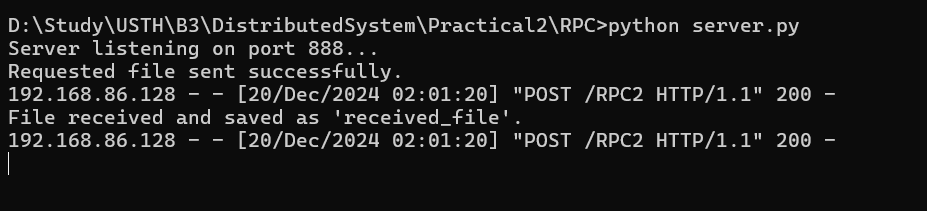
\includegraphics[scale=0.6]{test-server-2.png}
\end{figure}

\vspace{-0.7cm} % Adjust this value to set the space between figures

\begin{figure}[H]
    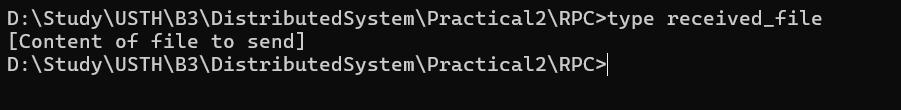
\includegraphics[scale=0.6]{test-server-3.png}
\end{figure}


\end{document}